\documentclass[journal,compsoc]{IEEEtran}

\usepackage{graphicx}
\usepackage{mathtools}
\usepackage{amsmath}
\usepackage{url}
\usepackage{listings}
\usepackage{float}
\usepackage{fancyvrb}
\usepackage{framed}
\usepackage{attrib}

\hyphenation{op-tical net-works semi-conduc-tor}

\newcommand{\ws}{WebSocket}



\begin{document}

\author{\IEEEauthorblockN{Thibault G\'erondal, Michael Heraly}}

\title{Survey paper: Websocket}

\date{Tuesday, 27 Oct 2015}

\maketitle
\IEEEpeerreviewmaketitle


%\IEEEdisplaynontitleabstractindextext

\begin{abstract}
The most common way to get some information and communicate through the internet is via the Hypertext Transfer Protocol (HTTP).
Over time, the shared media sent through this communication system have evolved.
It started from text to images and videos.
And interactions between clients and servers have evolved too.
We went from passive customers who receives informations to active clients that wants to communicate in real-time.
The original HTTP was never designed to achieve those needs.
The market found some tricks to bypass these limitations.
But the HTML5 initiative introduced a real solution to this problem : \ws{} JavaScript.
This solution brings socket to the web, so a full-duplex communication can be etablished between clients to the server.
% This paper is only bullshit, but let's try to sell it.
In this survey paper, we describe older techniques used that can achieve a full-duplex communication as \ws{} can do before describing \ws{} itself.
Then, we explore some experiments about how \ws{} is efficient compared to these older techniques.
Finally, a point is dedicated to the security issues of \ws.
\end{abstract}


\section{Introduction}

The Hypertext Transfer Protocol (HTTP) is a stateless request-response protocol in the server-client computing model. 
The client submits an HTTP request message and the server provides a response (HTML files, images, etc.) \cite{rfc2616}. 
With the evolution of the popularity of the web, applications have multiplied.
And the need of interactivity between the client and the server was increasingly felt. 
In the original HTTP specifications, interactivity was only possible by loading an entire page in order to upload information to the server or to receive new informations from the server.
But new features to web browsers have arisen in order to successfully add interactivity whithout (re)loading pages.
Among these, two Javascript API were were successively in web browsers : XMLHttpRequest and \ws.


\section{XMLHttpRequest}

One of the first and most used solution to add real-time interactivity is the XMLHttpRequest (XHR) Object which is a Javascript API that permits the browser to send a request for a ressource to a distant server.
Despite the name of this API, the fetched ressource don't have to be an XML file.
In fact, JSON (JavaScript Object Notation) is generally used as it is more easy to parse in Javascript.
This technique is great to send data to the server but not for receiving new data.
If the client want to keep up to date on information from the server, it will have to periodically poll the server.
However, doing  that generates a lot of overhead as each request will have a HTTP header and a lot of these requests might return no new data, so this technique is quite innefective.

\subsection{The long polling version}

The long polling also uses the XMLHttpRequest (XHR) Object. 
But, the client doesn't have to poll periodically the server as the web server hold the HTTP request open until it has new data to send to the client.
This reduces the amount of useless data transfers and improve the update delay as we can see in Fig.~\ref{poll_vs_lpoll}.

\begin{figure}
  \centering
  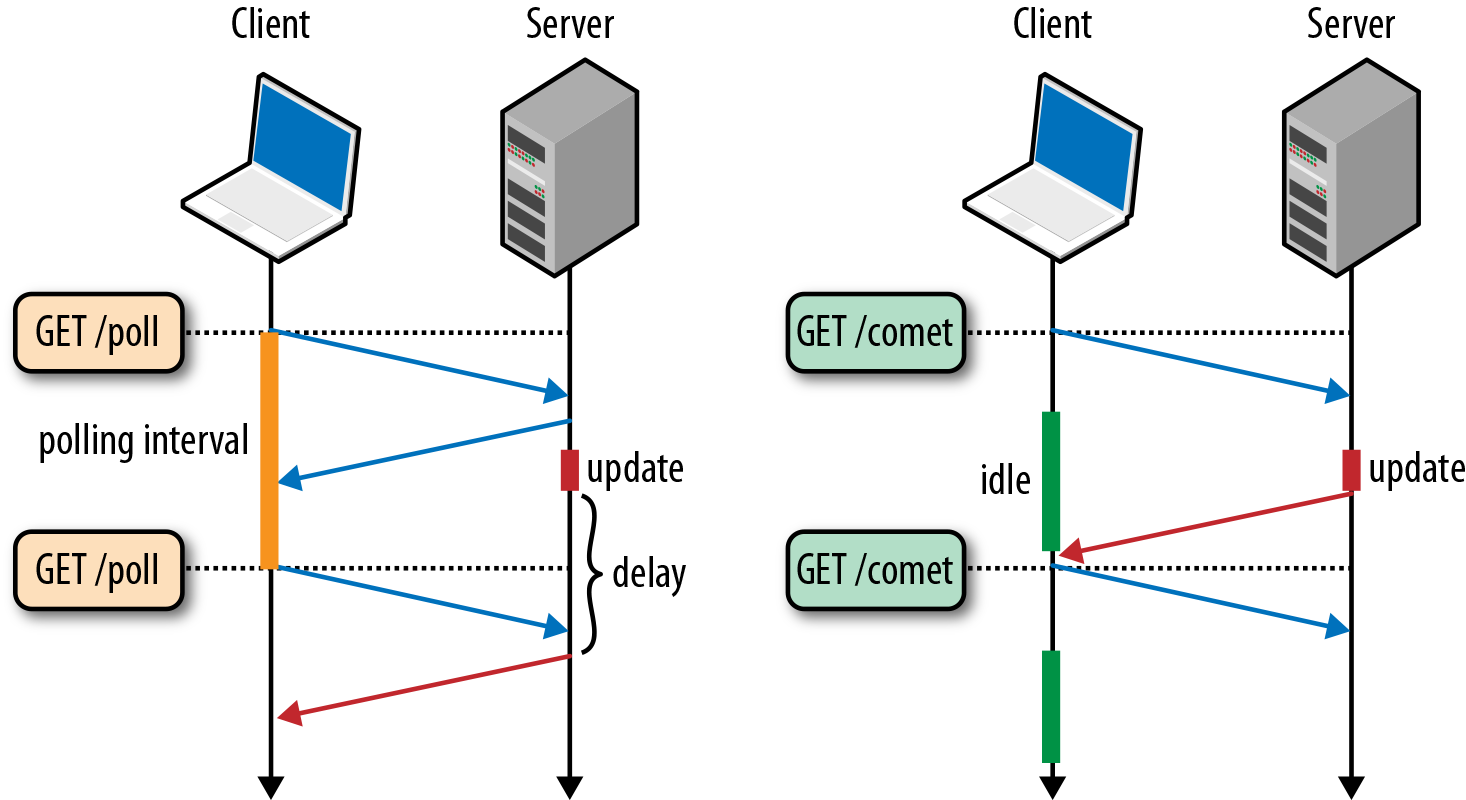
\includegraphics[width=\linewidth]{poll_vs_lpoll}
  \label{poll_vs_lpoll}
  \caption{periodic polling (left) versus long polling (right)}
\end{figure}

\section{\ws{} protocol}
The \ws{} protocol was standardized by the IETF as RFC 6455 in 2011 \cite{rfc6455}, and is being standardized by the World Wide Web Consortium (W3C).

 

\section{Performance of WebSocket}


\section{\ws protocol}



\subsection{Presentation}

\subsection{Concrete usage}

\section{Performance of \ws}

\subsection{Comparison with AJAX solutions}

\subsection{Behavior depending on the environment}

\section{Security}

\subsection{CORS}

\subsection{Proxies}

\section{Conclusion}

From a network point of view, \ws …


\ifCLASSOPTIONcaptionsoff
  \newpage
\fi


\bibliographystyle{IEEEtran}
\bibliography{bibi}


\end{document}
